\chapter{Implementierung}

\section{Distanzmessung}

Der Sensor von Pepperl+Fuchs wurde ursprünglich für die Distanzmessung angeschafft. Da dieser Sensor jedoch sehr teuer ist und wir nicht das Risiko eines möglichen Schadens im Vakuum eingehen wollten, wurde nach einer kostengünstigen Alternative gesucht.\\
Die Idee bestand darin, ein Entfernungsmessgerät von PARKSIDE zu verwenden und den Sensor aus dem Gerät zu entfernen. Die Messwerte werden anschließend mit einer MCU decodiert.

\subsection{Verbindung}
Der Sensor ist über ein Flachbandkabel mit der Hauptplatine verbunden, wie in Abbildung \ref{img_2_2:sen_dis_parkside:1} zu sehen ist. Auf der Hauptplatine befinden sich vier ungenutzte Lötstellen. Mithilfe eines Oszilloskops haben wir diese Lötstellen analysiert und festgestellt, dass Leitung eins eine Spannung von 3,3 V führt und Leitung vier als GND dient. Die Leitungen zwei und drei übertragen digitale Signale und fungieren als Datenleitungen.\\
Wenn zwei Leitungen für die Datenübertragung vorhanden sind, kann die Kommunikation bei einer zweiadrigen Verbindung entweder synchron oder asynchron erfolgen. Ist die Kommunikation synchron, dient eine der Leitungen als Taktleitung (Clock). Andernfalls, bei einer asynchronen Kommunikation, ist eine Leitung der Sender (TX) und die andere der Empfänger (RX). Dies ermöglicht eine Vollduplex-Übertragung.
Der Sensor komuniziert mit einem Bussystem. 




\begin{figure}[ht]
	\begin{center}
		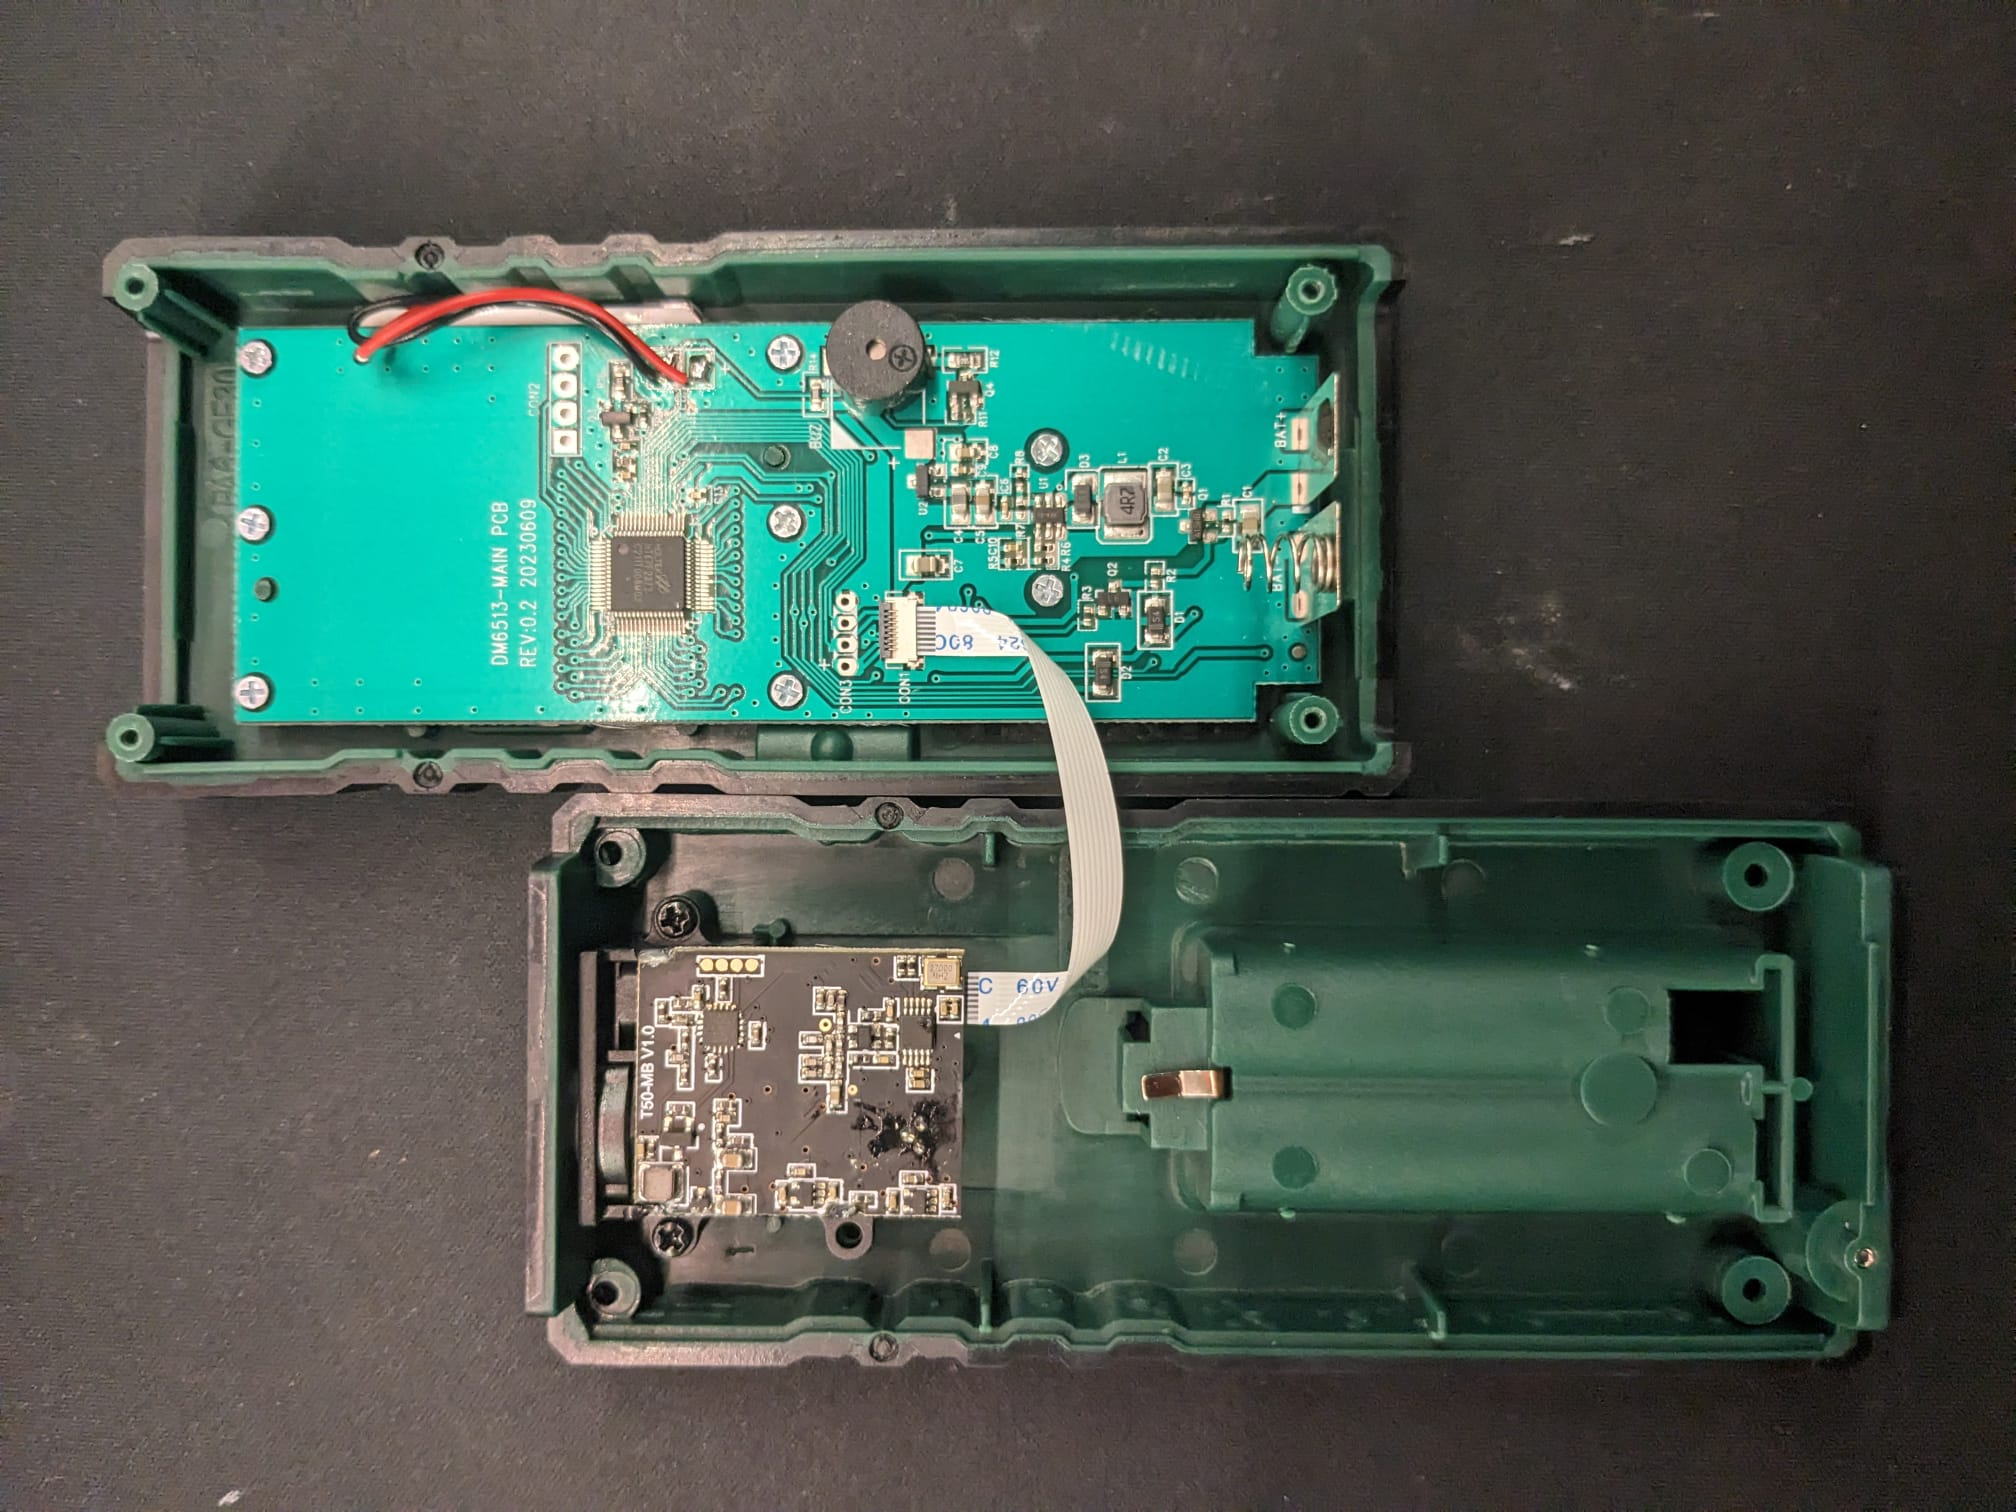
\includegraphics[width=1\textwidth]{img/2_sen/dis_parkside_1_outside.png}
		\caption{PARKSIDE – Distanzsensor – Innenaufbau}
		\label{img_2_2:sen_dis_parkside:1}
	\end{center}
\end{figure}


\begin{table}[ht]
	\centering
	\caption{PARKSIDE – Pin Mapping – Distanzsensor}
	\label{parkside:pinmapping}
	\begin{tabular}{l|ll}
		\hline
		\textbf{Pin} & \textbf{Farbe} & \textbf{Funktion} \\ \hline
		1            & Rot            & 3V3               \\
		2            & Weiß           & RX (receiver)     \\
		3            & Gelb           & TX (transmitter)  \\
		4            & Schwarz        & GND               \\ \hline
	\end{tabular}
\end{table}




\begin{itemize}
	\item + Anschlüsse herauszufinden vier anschlüsse gefunden.
	\item + Was für Aufgaben haben die Anschlüsse?
	      \subitem Was für ein Kommunikationsprotokol hat der Sensor?
	      \subitem Asynchron und seriell mit Baudrate 115200. (Ozilloskop)
	\item mit einem ESP32 die Sensordaten lesen.
	\item Nachrichtdekodierung (Controller MCU)
	      \subitem Ox24 Start (Nachricht start)
	      \subitem 0x26 Stopp (Nachricht ende)
	      \subitem 24 30 30 30 33 32 36 30 30 32 39 26 (Stopp signal)
	      \subitem 24 30 30 30 33 32 36 30 31 33 30 26 (Laser an)
	      \subitem 24 30 30 30 32 32 31 32 33 26 (Messen)
\end{itemize}


